%%%%%%%%%%%%%%%%%%%%%%%%%%%%%%%%%%%%%%%%%%%%%%%%%%%%%%%%%%%%%%%%%%%%%%%%%%%%%%%%%%%%%%%%%%%
%                               Related Work - 24-32pp
%%%%%%%%%%%%%%%%%%%%%%%%%%%%%%%%%%%%%%%%%%%%%%%%%%%%%%%%%%%%%%%%%%%%%%%%%%%%%%%%%%%%%%%%%%%
\chapter{Related Work}
\label{sec:RelatedWork}
 
\section*{Summary}

In this chapter, we will present the related work on IFC systems field. We will start by presenting an overview of IFC-related topics in Sect. \ref{sec:overview-ifc}. This overview consists in presenting the abstract IFC models in Sect. \ref{sec:ifc-models} and the IFC system design space, in Sect. \ref{sec:ifc-system-design-space}. After that, we will provide an insight over the most representative IFC systems operating on the mobile and server-sides, and also the distributed approaches, on Sect. \ref{sec:mobile-ifc-systems}, \ref{sec:server-ifc-systems} and \ref{sec:distributed-ifc-systems}, respectively. Finally, we will  summarize the related work with a brief discussion, on Sect. \ref{sec:related-work-discussion}.

The next chapter will introduce the proposed architecture of our system.

\section{Overview of Information Flow Control}
\label{sec:overview-ifc}

\todo{Say here again that we will present both models?}

\subsection{IFC Models}
\label{sec:ifc-models}

IFC is implemented in models that provide a way of defining meaningful parameters a given IFC system works according to. An IFC model defines how security policies are expressed in the system, how sensitive data is identified and labelled according to its source, and how the tracking of that data is achieved, to prevent unauthorized exfiltrations. The definition of an IFC model is a crucial part of our work, since the end-to-end protection mechanism Floodgate aims to achieve requires a well-defined IFC model that suits both mobile and server sides, relieving the integration issue. In this section we present two IFC models: The original IFC model that we refer to as Centralized Information Flow Control (CIFC) and Decentralized Information Flow Control (DIFC).

\subsubsection{Centralized Information Flow Control}
\label{sec:cifc-model}

Originally derived from military information management techniques, in which one unprivileged user can give information it owns to a privileged user but cannot have access to information owned by the privileged user (``no-read-up, no-write-down''), CIFC states that policies regarding who may access data are defined by an administration entity and enforced across the whole system. It enforces sensitive data protection by associating security labels with data and tracking the flow of information inside a program, avoiding the execution of actions that might compromise the privacy of this data.
The CIFC model also specifies principals. Principals represent entities (e.g., processes or users) that can interact with data. Labels are annotations that address both confidentiality and integrity constrains of data owned by principals, possibly defining different restrictions to each one. By labelling data, a more fine-grained control is achieved through different labels or set of labels for each purpose, forming a pair \texttt{\{confidentiality,integrity\}} assigned to a given data item. Confidentiality labels define the paths that data is allowed to flow to, while integrity labels constrain the paths where it is permitted to come from. Labels must be attached to data from the beginning and must not be removable or forged without the right permissions.
The labelling process, also called tainting process and illustrated in Fig. \ref{fig:cifc-model}, begins when there is an input of data into the system, possibly from direct user introduction (for example, UserA introduces a username and the corresponding password in a login form). This raw input generates untainted data (marked with \texttt{U}), which is data not analyzed by the labelling mechanism, and thus, not prepared to flow into the system. Untainted data is automatically forwarded to a taint source (represented as \texttt{TSrc}), a system component responsible for assigning a taint marking (represented as \texttt{T}) specifying the data type, and a confidentiality and integrity label, converting the raw data into tainted data (marked with \texttt{T}). Then, the now tainted data is introduced into the IFC system, being tracked across the program execution flow, the code that dictates the program's functionality. As data interacts with each other (i.e. passing values between variables) it results in exchanging labels to continue security enforcement, either increasing security-level (endorsement) or decreasing it (declassification). Finally, tainted data is verified at taint sinks (represented as \texttt{TSink}), normally network interfaces or database connectors, which mean points where data leaves the system, representing potential privacy threats.

\begin{figure}[t!]
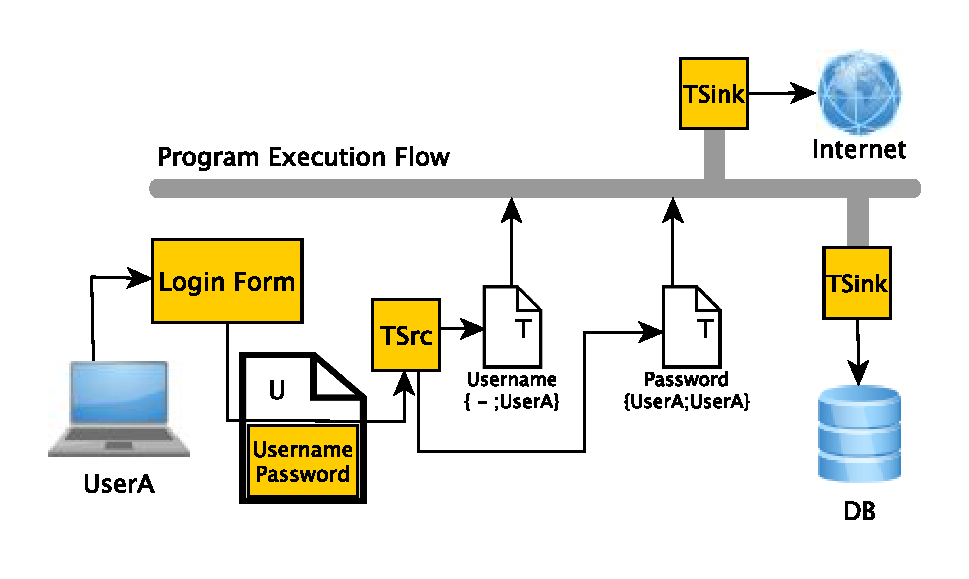
\includegraphics[width=0.7\textwidth]{figs/cifc-model}
\centering
\caption{CIFC operation scheme}
\label{fig:cifc-model}
\end{figure} 

For example, a label defined as \texttt{\{\{Alice;Bob\},Alice\}} would mean that both Alice and Bob are able to access data for read purposes but only Alice can alter this data. Also, the label \texttt{\{ - ,UserA\}} (as represented in Fig. \ref{fig:cifc-model} means that the associated data is public for read purposes but only \texttt{UserA} is able to alter it.
So, CIFC allows data-centric security policies to be defined by a central authority, specifying who can read or alter each data item in the system, allowing user's sensitive data to be protected against unauthorized accesses, therefore assuming the central authority responsible for policies definition is trusted and cannot be compromised.

\subsubsection{Decentralized Information Flow Control}
\label{sec:difc-model}
CIFC model described in Sect. \ref{sec:cifc-model} was primarily designed for simple environments where security policies are held and decided by a central authority, which enforces all the users to trust this system component, assuming that it cannot be compromised. It best suits systems where every operation is performed in the same single domain, thus not requiring data to be sent to untrusted third-parties. For example, a university where multiple departments coexist, being each department responsible for defining rules for data owned by itself. As we show below, this scenario cannot be modeled by CIFC, because there is no notion of data ownership, being a central authority responsible for controlling every access. Decentralized Information Flow Control \cite{difc} is a proposed model that improves CIFC by decentralizing the policy checking and holding from a central authority to the users themselves.

The essential parts of the DIFC model are: \textit{principals}, whose privacy the model is designed to protect; and \textit{labels}, the way in which principals specify their desired privacy constrains. DIFC labels, that take the form of \texttt{\{owner: readers\}} extend classic IFC labels by adding a notion of ownership to each label, which is a principal or group of principals that is able to declassify its own data but not to change policies held by other principals. Principals may delegate all their power in other principals, through acts-for relations specifying the new principals that can act on behalf of the original one.

Since these systems have to deal with information entering and leaving the system from/to remote locations, DIFC also extends these policy checks to the communication channels that support this data exchanges, associating them labels that operate on the input and output of data through these channels, with the purpose of not having any unlabelled data inside the system. When some value is read from an input channel, this value will be initially assigned with the label of the channel. On the other hand, a value can only be written to an output channel if the channel's label is at least as restrictive as the value's label, preventing this way information leaks through unprivileged communication channels.

DIFC base concepts and operation are demonstrated on Fig. \ref{fig:difc-model}, taking as example scenario an university management platform in which their students receive all the exam marks by e-mail. This example has the importance of showing how some common scenarios cannot be modeled by CIFC. The teacher corrects the exams, and when he finishes, he marks the exams as corrected. At this time, the exams are automatically sent to the university secretary that is responsible for sending the e-mails to the students with the corresponding marks. Also, the university has a private statistics bank where all the marks are compiled every year on performance reports that compare the students' success with previous years.

\begin{figure}[t!]
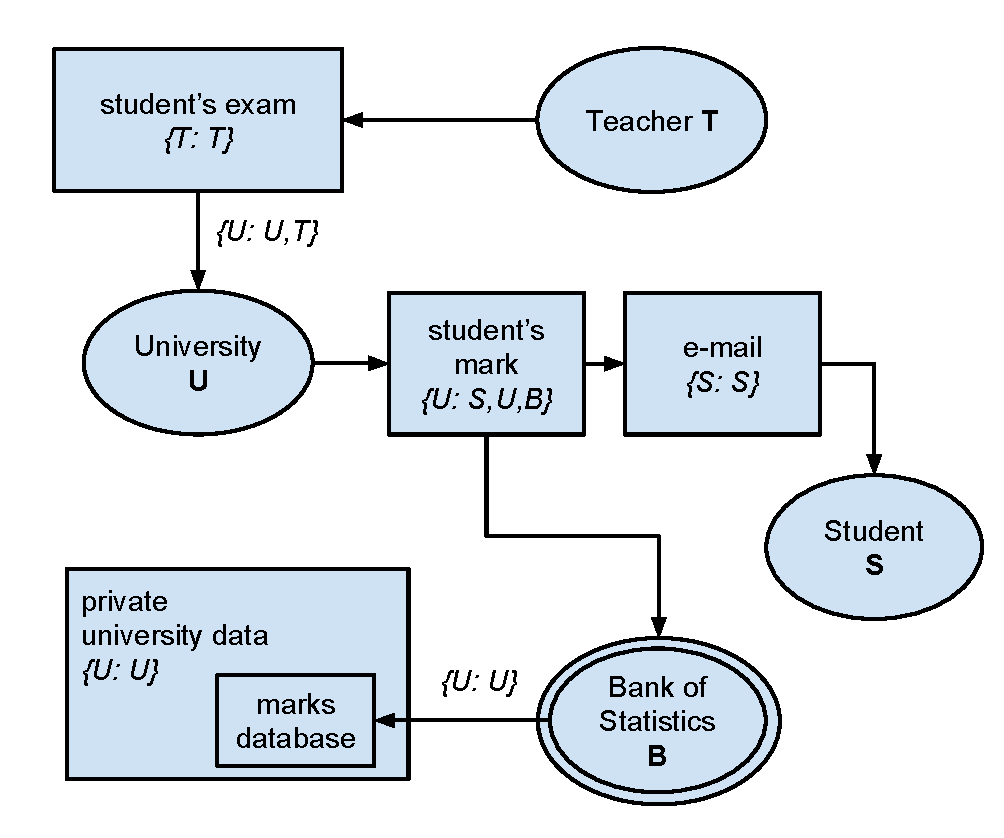
\includegraphics[width=0.7\textwidth]{figs/difc-model}
\centering
\caption{DIFC operation example}
\label{fig:difc-model}
\end{figure}

This is an example of a scenario where DIFC suits better than simple IFC, since the system is composed by multiple parts that not necessarily trust each other, as for example, a student may want to be sure that his marks are not leaked to other students. Also, a teacher may not want the university to be able to access the exam before he finishes the correction.

Modeling these restrictions in a DIFC model, we can find four principals, represent by ovals, which can hold data and need protection for that data: Teachers (\texttt{T}), University (\texttt{U}), that represents the university secretary, Student (\texttt{S}), and the Bank of Statistics (\texttt{B}) responsible for compiling and saving the statistics reports and which benefits from special trust by the university and the students, the reason why it's represented with a double oval.

The teacher corrects the exams, and when he finishes, the label \texttt{\{T: T\}} is assigned to the exam, specifying that the teacher is the owner of the exam and also only him is able to read it. When he finishes the correction, he gives the ownership of the exam to the university, but still keeps his ability to consult the exam. The university then takes the mark from the exam, composes an e-mail that is owned and only readable by the student \texttt{\{S: S\}} who will receive it, being sure that his information was not leaked anywhere else. Apart from that, the university makes the mark available for the bank of statistics to read, so it can be stored in the university database.

The bank of statistics has the authority to act on behalf of the university (\texttt{U}), so it can replace the student mark's policy from \texttt{\{U: U,B,S\}} to the statistics policy \texttt{\{U: U\}}, such that the mark can be saved in the statistics database and only accessible by the university.

In this scenario, there occur declassification in four situations. In first place, when the teacher transfers the exams ownership from himself to the university to process them. Then, the university composes an e-mail to be sent to each student carrying his mark, declassifying the e-mail to be owned and readable by the student only. At the same time, the university declassifies the mark, making it available for the bank of statistics to read, in order to include it in the yearly report. Finally, the bank of statistics endorses the mark's security, transferring the ownership of the mark to the university again, so it can be stored in the private database. In each situation, we are applying the rule that a principal may only modify the policies owned by itself, not present in centralized information flow control, which is the reason why it cannot model this scenario.

\subsubsection{Discussion}
In this section, we discuss which of the presented information flow control models better suits our mobile application target scenario.

Multiple similarities can be spotted between this scenario that suits the DIFC model for privacy protection and the examples of applications that exchange sensitive information about their users and that we approach as targets for the Floodgate. Foremost, the multiple principals that comprise the scenarios can be compared as current applications that rely on multiple third-party services where each one has the responsibility for a part of the whole system functionality and does not necessarily trust the others.

For example, a mobile application that presents location-based suggestions to its users may query a restaurants database for suggestions of where to eat and a monuments database to find the best places to visit. Apart from that, it may still require advertisements from another third-party server, so we consider each one of these parties as a principal in the model. A distrustful relationship is present, since the user may not trust the third-party content providers and these may not trust the application itself.

To address this trust issue, the DIFC system must possess data declassification mechanisms that allow principals to constantly exchanging privileges over information, granting or removing permission to/from other principals to access data. For example, the user location must be protected from third-party leaks, and thus, the user could define that only him and the principals that need to access its location to proffer functionality may access this information. For this reason, we argue that the DIFC model best fits our needs in terms of data tracking, policies specification and enforcement, and so must be seen as good basis for the Floodgate system model.

\subsection{IFC System Design Space}
\label{sec:ifc-system-design-space}

Since the concept of IFC was proposed, multiple systems and techniques emerged, differing between them on key design issues, which, according to Bacon et al. \cite{bacon2014}, can be summarized on the following questions:

\begin{enumerate}
\item When the system operates?%(static, runtime, hybrid);
\item Which granularity the system operates at?% (e.g. domain level, process level, variable level, message level);
\item How the system enforces data isolation?% (hardware-assisted OS, programming language libraries);
\item How the system specifies data policies?
\end{enumerate}

\subsubsection{1. When the IFC System Operates?}
An IFC system may be a static method if its operation occurs at the program compilation time or a runtime method if it operates dynamically when the program is running, accepting data exchanges in and out of the system. Finally, a hybrid method comprises at least two components, extending the method operation at both compilation time and runtime.

\textbf{Static methods} provide a way to verify the correctness of cloud components and all the interactions that happen between them. These mechanisms allow cloud providers to guarantee a trusted base on top of which their clients can deploy applications. Despite they are not effective in enforcing end-to-end privacy protection on runtime, during dynamic arrival of application inputs, these methods are immune to IFC threats like timing or termination channels. As examples of static methods we outline:

\textbf{Static taint analysis}, implemented in Pixy \cite{pixy}, a technique that analyses a target program in order to check that every accepted input is sanitized before it can be considered as safe to be applied in the system operation. It attempts to prevent attacks like SQL injection or Cross-Site Scripting (XSS) \cite{xss}. Also, \textbf{security-Typed Languages}, such as Haskell \cite{haskell}, allow application developers to explicitly define security policies attached to the type of each variable while writing the application code. The compiler enforces to take these confidentiality and integrity policies at program compilation time.

\textbf{Runtime IFC methods} are techniques to achieve data labelling and taint tracking while a program is running. Despite they add a runtime overhead due to the taint tracking mechanisms, these systems are able to detect potential dangerous information flows, in which sensitive information belonging to users might be leaked or malicious data might damage the system itself.

TaintDroid \cite{taintdroid} is an example of a runtime method, which monitors Android applications while running. It detects when applications try to exfiltrate data coming from sensitive information sources (i.e., device location sensor, user phonebook), reporting the responsible application, data type and network destination to the user.

Apart from purely static and purely runtime systems exemplified above, there are special cases known as \textbf{hybrid methods} because of their operation both at compile and runtime.

Jif \cite{jif} must be seen as a hybrid system that divides its functionalities between both compile and runtime. Jif is an example of a security-typed language which extends Java by adding DIFC labels to the data type system. These labels define a set of rules that a program must follow in order to prevent sensitive data leaks. Then the compiler verifies all program statements based on DIFC labels, which include compile-time checks (static component) of whether data with a certain associated label reaches another variable or a communication channel associated with a more permissive label, generating compilation errors in such case. Apart from that, Jif allows ownership and permissions over data to be granted and checked by the system in runtime, which is useful in systems where information flow cannot be verified statically and privileges over information may change over time.

\subsubsection{2. Which Granularity the System Operates at?}

Current IFC systems often divide an application into multiple isolated components that vary on their contribution to the whole application and on the security-level required to interact with them. Generally, data inside an application flows across isolated components, possibly exchanging labels and metadata on each transition, so it is essential to intercept the exchange of data, analyze the intercepted data and update information flow metadata accordingly, if necessary. IFC tracking can be enforced at different granularities and systems must determine a balanced way of providing effective data tracking while minimizing additional verified overhead.

\paragraph{A) Tracking at VM Level:}
Considering an architecture where multiple virtual machines controlled by a hypervisor run different applications, there is the need to control how data flows between virtual machines and also interactions with the hypervisor. Payne et al. \cite{payne} proposed a layered model for security policies, in which every request between VMs running over the same hypervisor is associated with two labels. One label is assigned by a guard component responsible for inspecting the request type and content, and the other one, derived from the first, is assigned by the hypervisor stating whether the request may reach the destination VM. This distribution is done in order to lower complexity by reducing the relations verified at each layer.

\paragraph{B) Tracking at Process Level:}
A fine-grained approach, tracking at process level allows taint tracking to intersect and verify data exchanges between different applications installed on the same device, requiring each one to be encapsulated on its own process. This way, every interaction between different processes is intercepted and analyzed by the data flow tracking system. It is used in Asbestos \cite{asbestos}, Flume \cite{flume}, HiStar \cite{histar}, Nexus \cite{nexus}, Laminar \cite{laminar}, DStar \cite{dstar} and almost all DIFC-driven operating systems, but also suffers from little adoption since it requires a deep change on the application's development environment and it is not capable of tracking suspicious interactions within the same software component as a variable-level approach do.

\paragraph{C) Tracking at Variable Level:}
Providing data flow tracking at variable level, allows every variable defined in the context of an application to be monitored, preventing unsafe uses. Jif \cite{jif} language attaches to each variable a pair of labels composed by a confidentiality label and an integrity label. These labels are checked on each interaction between components and data holding them may be endorsed or declassified, based on the privacy needs at each moment, defining the possible flows an application can securely allow. Even in the presence of incorrect or malicious software implementations, if labelling is correctly defined, a user trying to read another's confidential data will be presented with an exception indicating the invalid request made.

\paragraph{D) Tracking at Multiple Levels:}
IFC systems designed to operate exclusively at mobile side usually combine multiple of these approaches to achieve an efficient data tracking. Uppermost, the OS running on mobile devices is slightly different from general Linux distributions widely used to power servers on which applications base their functionality. Also, contrary to what happens on Linux, applications running on mobile operating systems must be written in one specific language that provide interfaces to communicate with the device itself, in order to gather information. On Android systems, applications are written in a modified version of Java language, and thus, IFC systems designed to operate over Android \cite{taintdroid,pebbles,mockdroid} know a priori which language libraries and variables to track. Apart from variable/library-level tracking, Android-supported IFC systems also perform tracking at interprocess message-level, since each application runs on its own Dalvik VM encapsulated in a process, which results in a way of controlling how taints are propagated between applications. Finally, as every Android device runs its own filesystem where application data is often persistently stored in files, these systems also perform tracking at file-level, keeping security labels hooked to the corresponding files. This file-level tracking is crucial for the system effectiveness because files often contain much more information than variables. In conclusion, mobile IFC systems maintain users privacy by acting as all-around privacy protection mechanisms for mobile devices.

\subsubsection{3. How the System Enforces Data Isolation?}
Data isolation is an essential mechanism to complement data flow tracking and analysis, since it prevents data from being exported through unexpected channels or flowing into undesired system components without previous security monitoring and sanitization. For example, a secure container encapsulates the execution of an application so that data is securely accessed and input/output is checked for security purposes. The goal of data isolation mechanisms is to only allow data exchange when the application requirements strictly need it. To achieve data isolation, the following approaches have been studied:

\paragraph{A) Isolation Through Virtualization:}
On a virtualized environment, isolation is performed at the virtual machine level and enforced by both the hardware and the hypervisor. The CLAMP system \cite{clamp} provides a virtualized environment to applications built under the popular Linux, Apache, MySQL, PHP/Perl (LAMP) stack, allowing developers to continue using the operating systems, platforms and languages they are used to. CLAMP uses the Xen hypervisor to isolate each user's data on a virtual dedicated web server instance, only accessible through authentication on a developed module. The database queries performed by the user are restricted a trusted Query Restrictor that guarantees that only data owned by the user assigned to the querying web server can be accessed.

\paragraph{B) Isolation Through Programming Languages and Libraries:}
In opposition to isolation achieved at the VM-level, recent implementations of IFC systems allow developers to explore the taint-tracking facilities present in languages like Ruby and Perl to enforce data isolation at the best possible, since it cannot be strictly enforced. These approaches have the advantages of isolating data just by interacting with already defined language libraries, discarding the need to adapt the runtime environment to accommodate desired isolation features. SAFE WEB \cite{safeweb} uses Ruby dynamic features, like safe levels. Safe levels can restrict the execution mode of Ruby code on different kinds of isolated environments, through a \$SAFE variable that has 4 isolation levels (level 4 means no I/O operations). Relying on this, SAFE WEB achieves label propagation and data flow enforcement, but it is primarily suitable for detection and protection against unintentional software bugs than to deal with explicitly malicious application code from unreliable third-party providers.

\paragraph{C) Isolation at \textit{Middleware} Level:}
Designed for multi-tier web applications in which data has to flow between multiple sub-systems, called domains, event-based IFC systems define messages between these domains as events. SAFE WEB is an example of an event-based IFC system which apply an event-level or message-level granularity in data flow isolation. In these type of systems, events between domains are often placed in an event broker by the sender domain, and the event broker handles the task of delivering events only to interested domains that are allowed to read the event information, being this event broker the only way how domains are able to exchange messages.

\subsubsection{4. How the System Specifies Data Security Policies?}
A basis option to take in the designing of an IFC system is to specify how security policies are unambiguously defined. Currently used examples are policy-definition languages or \textit{ad-hoc} definitions, specific to each system. 

\paragraph{A) Policy-Definition Languages:}

Policy-definition languages allow the specification of ``can-flow-to'' relations between DIFC labels, applicable in the context of every application, just by having the knowledge of principals present in the application. JFlow \cite{jflow} is a policy-definition extension for Java language that allows the programmer to define allowed relations between labels under a usable programming model, making it simple to use.

\paragraph{B) \textit{Ad-hoc} Policy Definition:}
In contrary to what happens with the usage of languages to specify security policies, an ad-hoc policy definition means that security policies are specified by the developer itself, that is responsible for writing policy checking code. RESIN \cite{resin}, is an example of an \textit{ad-hoc} policy definition system, allowing programmers to create \textit{policy objects}, which specify assertions associated with application data to be checked when data crosses certain data flow boundaries (i.e., in an attempt to send data over the network).

Throughout the time, there emerged some real systems that implement the IFC models described above. We now present the most representative cases, based on Floodgate's context which implicates three different types: Systems which operate on the mobile-side only, others that do it exclusively on the server-side and also the distributed approaches, which implicate data communication between two entities. 

\section{Mobile-side IFC Systems}
\label{sec:mobile-ifc-systems}

For the mobile-side, we chose three systems which take different approaches: TaintDroid, Aurasium and FlowDroid.

\textbf{TaintDroid} is an extension to the Android mobile operating system capable of tracking the flow of sensitive data across downloaded third-party applications. TaintDroid aims at informing mobile devices' users of how these applications make use of permissions granted on installation.

TaintDroid regards two main goals: The detection of when sensitive data, like user's location or information about the device, leaves the system through third-party applications that might send it to remote locations on the network. The other one is to facilitate application security analysis by device users or external security auditors. With TaintDroid, a user can easily verify whether an application performs active intents to leak its private data.

An approach through static source-code analysis is infeasible, because most applications are closed source and often are realtime changeable configurations that dictate application's behavior. So, TaintDroid uses \textit{dynamic taint analysis} to monitor privacy sensitive data on mobile devices. TaintDroid knows \textit{a priori} the sets of taint sources and sinks present in the device.

Firstly, information coming from a \textit{taint source} (source of sensitive information, like the GPS sensor) is identified and a \textit{taint marking} indicating the information type (location-sensitive, contact-sensitive) is assigned. Then, dynamic taint analysis perform an instruction-level tracking on how labelled data interacts with other data over the application information flow in a way that might cause the leakage of the original data. Finally, all the impacted data is identified when an intent of leaving the system through a \textit{taint sink} (normally the network interface) is detected.

Taking advantage of virtual-machine-based smartphones architectural characteristics, TaintDroid provides an efficient, system-wide taint tracking mechanism, illustrated in Fig. \ref{fig:taintdroid-arch}. In first place, the VM interpreter is instrumented to provide \textit{variable-level} tracking within the application code. Then, \textit{message-level} tracking between applications is used, since applications are allowed to share data between themselves through Binder, i.e., the Android component responsible for IPC. Third, for trusted system-native libraries, TaintDroid uses \textit{method-level} tracking, running code without instrumentation and applying the taint propagation on the method return. Finally, \textit{file-level} tracking is used to ensure that information stored persistently also keeps the assigned taint markings.

\begin{figure}[t!]
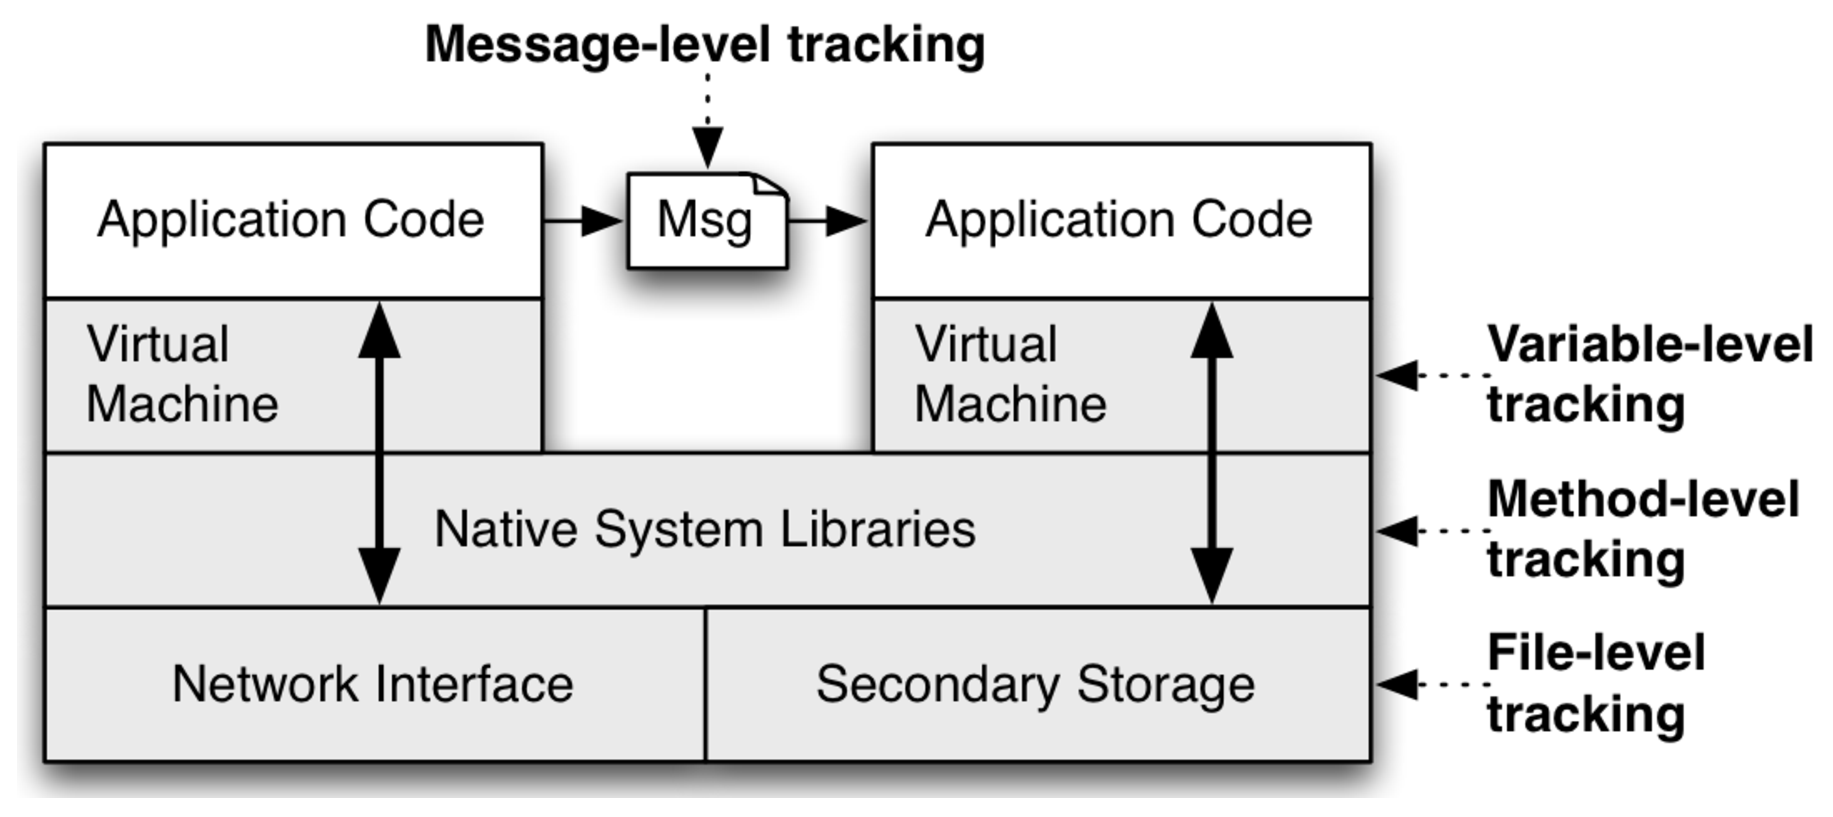
\includegraphics[width=0.7\textwidth]{figs/taintdroid-arch}
\centering
\caption{TaintDroid tracking system overview}
\label{fig:taintdroid-arch}
\end{figure}

To ensure that applications are not capable of maintain sensitive untracked data flowing in the system, TaintDroid assumes that the TCB is comprised only by the virtual machine (not the code) executed in user-space where applications operate in and the operating system, or more specifically any native system libraries loaded by the untrusted interpreted application. This way, TaintDroid modified the original Android platform to only allow applications to escape the virtual machine through native libraries that are, therefore, trusted.

Figure \ref{fig:taintdroid-arch-2} gives a detailed view over the TaintDroid architecture. After information is tainted (1) on a trusted application that carries enough context to perform the taint operation (the location-provider, for example), the taint interface invokes a native method (2) that interacts with the Dalvik VM interpreter, storing some specified taint markings in the \textbf{virtual taint map}. The Dalvik VM is then responsible for propagating taint tags (3) according to data flow rules, while the application uses the tainted data in its operations. Multiple interpreters may be propagating taint information, as many applications may be running at the same time. By the time that the trusted application uses the tainted information in an IPC call, the Binder IPC Library (4) ensures that the data archive containing all data to be transferred has a \textbf{taint tag} reflecting all the taint markings of all associated data. If true, the Binder Kernel Module (5) performs the dispatch of the data, which will be received by the IPC library on the untrusted application side. This library then removes the taint tag from the data archive and assigns it to every data contained in it. The Dalvik VM interpreter then propagates the taint markings (7) on the untrusted application side, identically to what happens on the trusted side and anytime the untrusted application invokes a library (8) known as part of the taint sinks set (e.g. network interface), this library reads the taint tag from data referred in the invocation (9) and reports the event, describing the exported data, its destination and the associated taint tag.

\begin{figure}[t!]
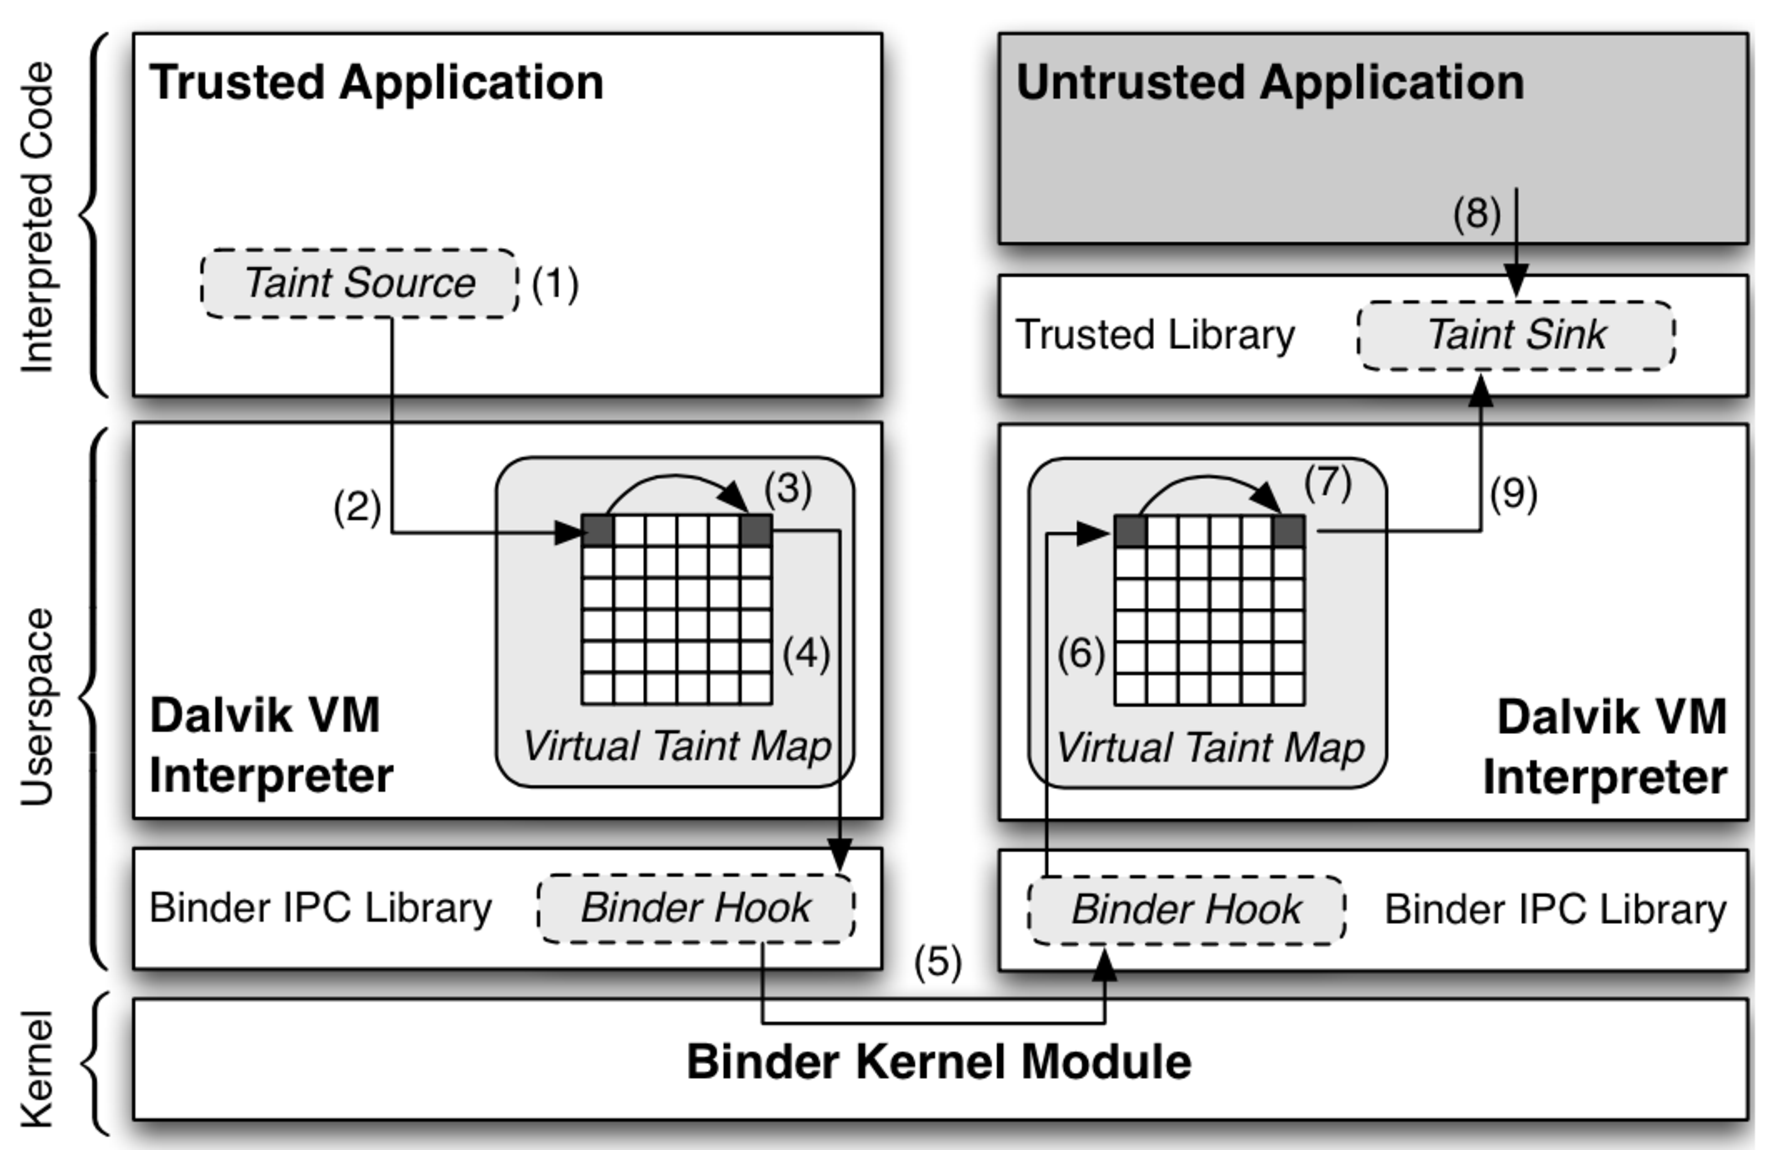
\includegraphics[width=0.7\textwidth]{figs/taintdroid-arch-2}
\centering
\caption{TaintDroid architecture}
\label{fig:taintdroid-arch-2}
\end{figure}

TaintDroid stores taint tags in memory positions adjacent to variables, like class fields or arrays, providing spatial locality that might influence the system performance positively. Also, only one taint tag is stored per array, which minimizes storage overhead but may lead to false positives, since if an array contains only one tainted data object in a given position, the whole array must be considered as tainted.

Against the stock Android platform, TaintDroid revealed a 3\% performance overhead in starting an application, 5.5\% and 18\% increased time for address book create and read operations, respectively, 10\% overhead in making a phone call and 29\% overhead on taking a picture with the device camera. Also, an IPC benchmark revealed that for a set of 10.000 messages exchanged between client and server applications performing binder transactions, TaintDroid is 27\% slower and uses 3.5\% more memory.

TaintDroid presents an efficient approach to track information flows on Android systems. The dynamic taint analysis method offers effectiveness on tracking how information coming from taint sources are used throughout the application, relieving the need to trust the application itself. Also, the spatial locality provided by the taint tag storage method minimizes the added overhead. Although, TaintDroid is not effective in preventing the exfiltration of sensitive data, since it only builds a report of situations when it occurs, instead of blocking network access in such cases, which is included in Floodgate's goals.

The second mobile IFC system we present is \textbf{Aurasium}, which may be described as an application-hardening service. It is intended to be used in order to turn untrusted Android applications, downloaded from third-party providers, into secure applications enforcing policies regarding the user's sensitive data privacy. In order to achieve that, the system relies on a repackaging process of the application package, and the output is a hardened version of the same inputted application to be directly installed on a device.

In practice, Aurasium takes advantage of Android's application design of mixed Java and native code execution to introduce \textit{libc} interposition code to the target application, wrapping around the Dalvik VM under which the application's Java code runs. This way, Aurasium is able to intercept almost all interactions between the application and the operating system, since most of them trigger the execution of native methods, which is often transparent to developers, due to the available APIs. Also, code modification is used in order to place the interposition code whenever the application starts. Figure \ref{fig:aurasium-arch} illustrates the space where the system acts in the Android OS context.

\begin{figure}[t!]
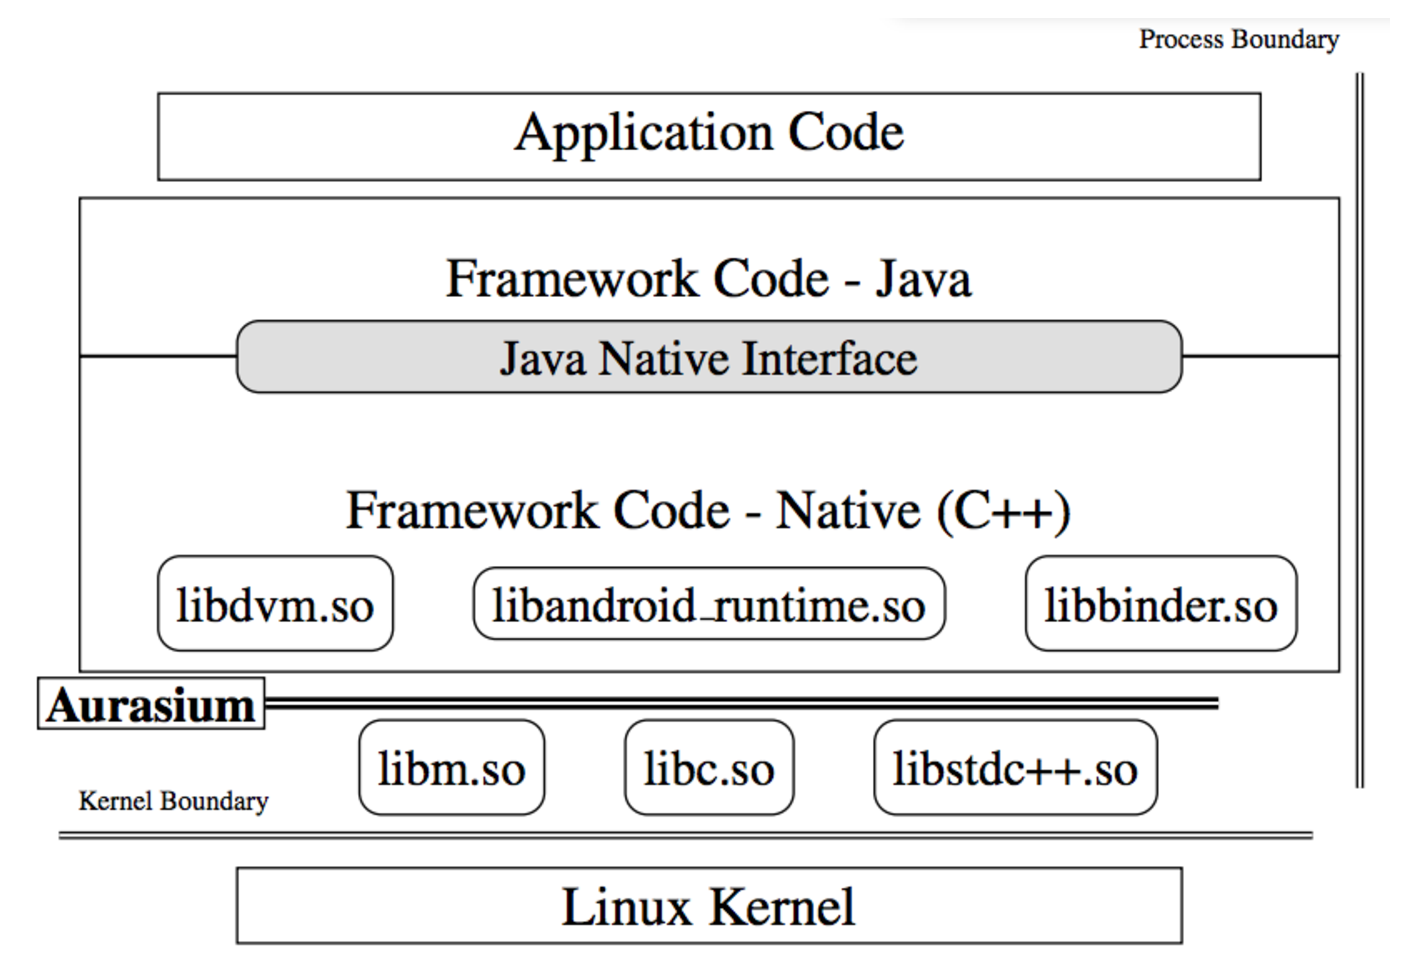
\includegraphics[width=0.7\textwidth]{figs/aurasium-arch}
\centering
\caption{Aurasium action context}
\label{fig:aurasium-arch}
\end{figure}

In Aurasium, the security policies are enforced, for example, whenever an application tries to communicate with a remote endpoint through the network. In such case, Aurasium first checks it against an well-known IP blacklist, frequently updated. Also, whenever an application
tries to access the device's IMEI, as illustrated in Fig.  \ref{fig:aurasium-policy}, a policy check is performed to allow or disallow the access. These policies are included in the self-contained final application package and may save its state and check it in future occasions. Aurasium's interposition code shows a dialog to the user, asking whether permission to perform an action which might violate the security policies should be granted.

\begin{figure}[t!]
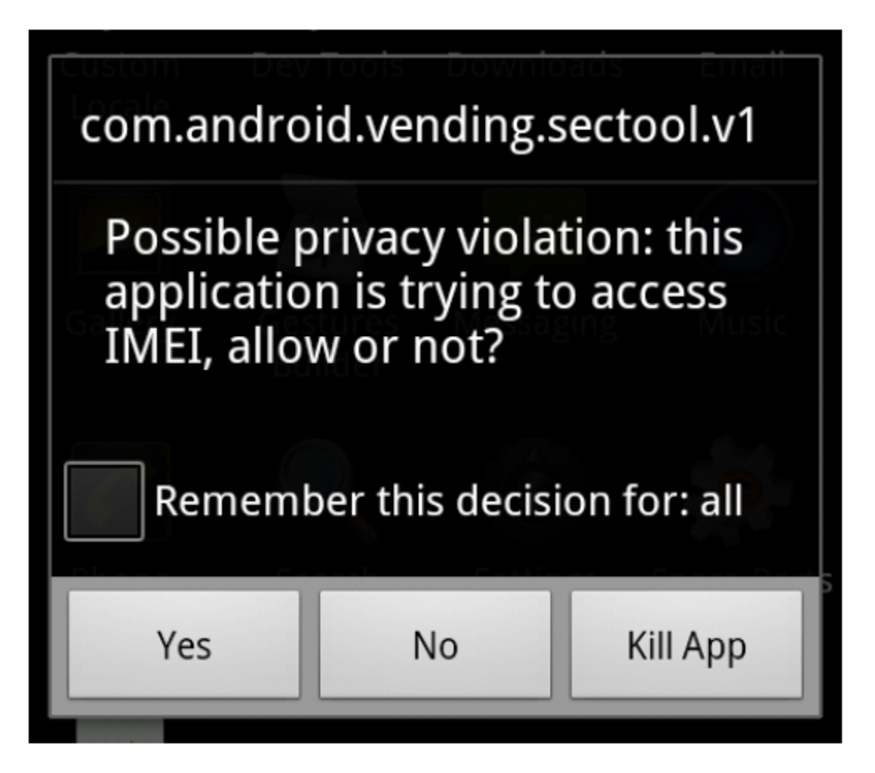
\includegraphics[width=0.5\textwidth]{figs/aurasium-policy}
\centering
\caption{Aurasium policy example}
\label{fig:aurasium-policy}
\end{figure}

In order to produce the hardened version of an application to be run in the same devices as its non-secure version, Aurasium first needs to decompile the application's compiled bytecode, which is stored in a single file called \texttt{classes.dex} inside the application's \texttt{APK} package. After that, the code is inserted in normal Java classes and the application entry point is set to the Aurasium \texttt{Application} class, which guarantees that Aurasium becomes the application's entry point and its sandbox is established before the application can perform any other action. Figure \ref{fig:aurasium-repackaging} shows the components of a common \texttt{APK} package and the Aurasium components introduced during the repackaging process.

\begin{figure}[t!]
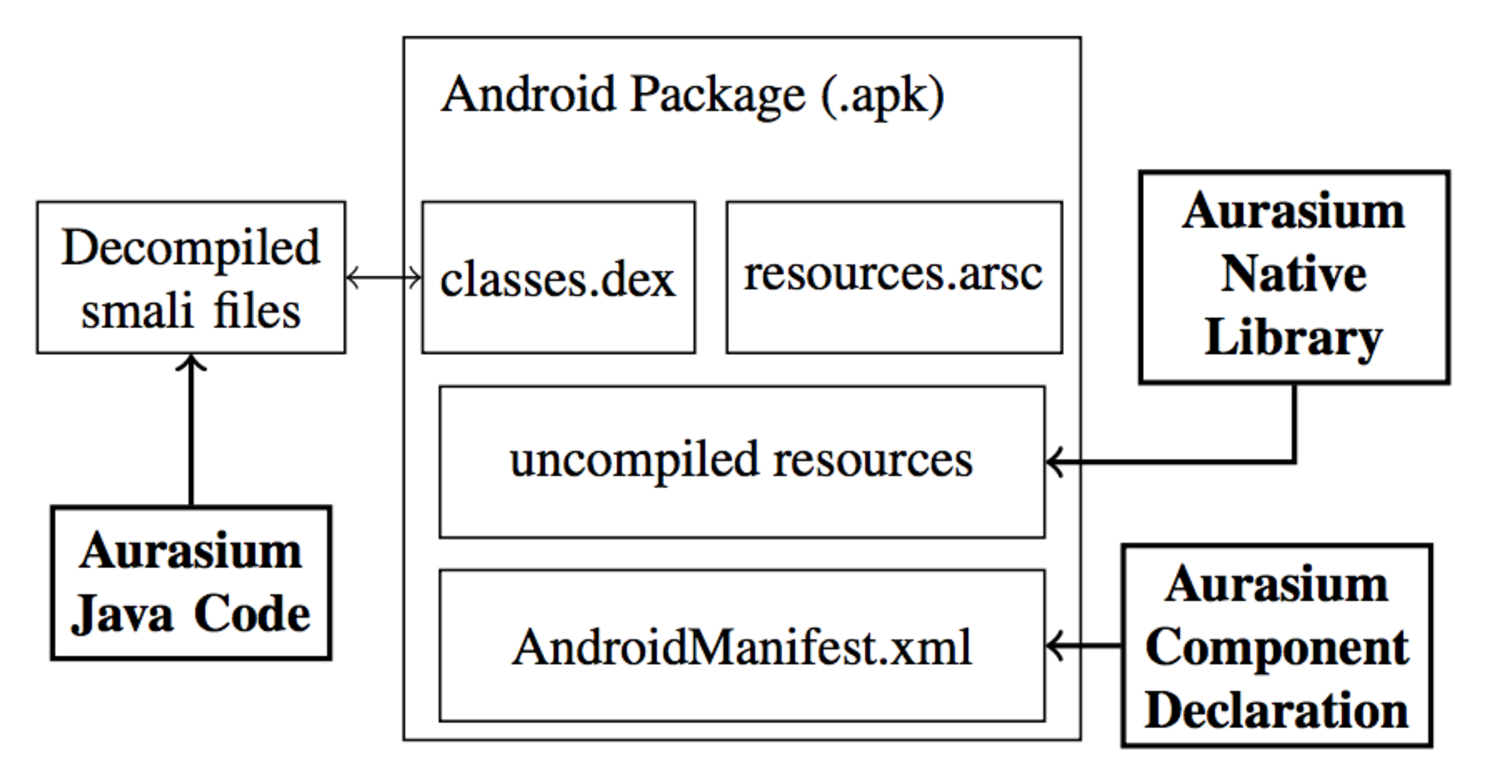
\includegraphics[width=0.7\textwidth]{figs/aurasium-repackaging}
\centering
\caption{Aurasium repackaging process}
\label{fig:aurasium-repackaging}
\end{figure}

After the repackaging process, the final step is resigning the application package, since every Android application is required to have a valid signature, which proves its authorship. To maintain this, Aurasium keeps the application's old signature (before the repackaging), and then verifies its validity. If it is valid, then the application is re-signed with its old signature. If don't, then Aurasium will use a randomly-created signature, which will not keep the application's authorship information.

To complement, Aurasium features a helper application, named Aurasium Security Manager, which users may install in order to centrally manage permissions granted/revoked to their Aurasium-packaged applications. For instance, if a user permanently decided to not let a given application access his phone number, with this helper application they may change it in the future.

In terms of performance, Aurasium shows worse results when applications perform a large number of requests to the underlying Android APIs, with an overhead of 14\% to 35\% on three use-cases, specifically developed to perform a lot of API invocations. In terms of size of the hardened application package, Aurasium showed a constant increasing of about 52 Kb, which the authors considered a minor overhead.

In conclusion, Aurasium tries to achieve practical security enforcement and contributes with its novel repackaging process and a set of policies regarding sensitive mobile information. This system shares with Floodgate the goal of not requiring changes on the mobile operating system in change for protection, avoiding problems regarding the system's adoption and cross-version compatibility.

The third mobile IFC system we present is \textbf{FlowDroid} \cite{flowdroid}.

\section{Server-side IFC Systems}
\label{sec:server-ifc-systems}

\section{Distributed Approaches}
\label{sec:distributed-ifc-systems}

\section{Discussion}
\label{sec:related-work-discussion}
 
 
